
\appendix
\chapter{Further Properties of the Geometric Product}\label{Appendix_A}
For two vectors $a$ and $b$ we can revise the order of the geometric product via the formula
\be\label{x1}
	ba = 2a\cdot b-ab.
\ee
By repeated applications of equation~\ref{x1} we can relate the geometric product $aa_{1}\dots a_{r}$ to the geometric product $a_{1}\dots a_{r}a$ -
\begin{align}
	aa_{1}\dots a_{r} &= 2\paren{a\cdot a_{1}}a_{2}\dots a_{r}-a_{1}aa_{2}\dots a_{r} \nonumber \\
	                  &= 2\paren{a\cdot a_{1}}a_{2}\dots a_{r}-2\paren{a\cdot a_{2}}a_{1}a_{3}\dots a_{r}+a_{1}a_{2}aa_{3}\dots a_{r} \nonumber \\
	                  &= 2\sum_{k=1}^{r}\onep{k+1}\paren{a\cdot a_{k}}a_{1}\dots \breve{a}_{k}\dots a_{r}+\onep{r}a_{1}\dots a_{r}a.\label{x2}
\end{align} 
Thus
\begin{align}
	\half\paren{aa_{1}\dots a_{r}-\onep{r}a_{1}\dots a_{r}a} &= \sum_{k=1}^{r}\onep{k+1}\paren{a\cdot a_{k}}a_{1}\dots \breve{a}_{k}\dots a_{r} \nonumber \\
	                         a\cdot\paren{a_{1}\dots a_{r}}  &= \sum_{k=1}^{r}\onep{k+1}\paren{a\cdot a_{k}}a_{1}\dots \breve{a}_{k}\dots a_{r}. \label{x4} 
\end{align} 

Now consider the expression $a\cdot\paren{a_{1}\W\dots\W a_{r}}$ and how it can be reduced.  Since $a_{1}\W\dots\W a_{r}$ only contains grades $r$, $r-2$, $\dots$,
we have
\begin{align}
	a\cdot\paren{a_{1}\dots a_{r}} &= \half\paren{aa_{1}\dots a_{r}-\onep{r}a_{1}\dots a_{r}a} \nonumber \\
	                               &= a\cdot\grd{a_{1}\dots a_{r}}{r}+a\cdot\grd{a_{1}\dots a_{r}}{r-2}+\cdots
\end{align}
The term we need is the $r-1$ grade part so that
\begin{align}
	a\cdot\paren{a_{1}\W\dots\W a_{r}} &= \half\grd{aa_{1}\dots a_{r}-\onep{r}a_{1}\dots a_{r}a}{r-1} \nonumber \\
	                                   &= \sum_{k=1}^{r}\onep{k+1}\paren{a\cdot a_{k}}\grd{a_{1}\dots \breve{a}_{k}\dots a_{r}}{r-1} \nonumber \\
	                                   &= \sum_{k=1}^{r}\onep{k+1}\paren{a\cdot a_{k}}\paren{a_{1}\W\dots \W\breve{a}_{k}\W\dots\W a_{r}} \nn \\
	                                   &= \sum_{k=1}^{r}\onep{k-1}\paren{a\cdot a_{k}}\paren{a_{1}\W\dots \W\breve{a}_{k}\W\dots\W a_{r}}. \label{eqA_5}
\end{align}

If $A_{r}$, $B_{s}$, and $C_{t}$ are pure grade multivectors of grade $r$, $s$, and $t$ we have
\begin{align}
	A_{r}\cdot\paren{B_{s}\cdot C_{t}} &= \paren{A_{r}\W B_{s}}\cdot C_{t} \;\forall\; r+s\le t \mbox{ and } r,s > 0 \label{eqA_6}\\
	A_{r}\cdot\paren{B_{s}\cdot C_{t}} &= \paren{A_{r}\cdot B_{s}}\cdot C_{t} \;\forall\; r+t\le s \label{eqA_7}.
\end{align} 
To prove equation~\ref{eqA_6}
\begin{align}
	A_{r}\cdot\paren{B_{s}\cdot C_{t}} &= A_{r}\cdot\grade{B_{s}C_{t}}{t-s} \nn \\
	                                   &= \grade{A_{r}\grade{B_{s}C_{t}}{t-s}}{t-\paren{r+s}} \nn \\
	                                   &= \grade{\grade{A_{r}B_{s}C_{t}}{t-\paren{r+s}}+\mbox{higher grades}}{t-\paren{r+s}} \nn \\
	                                   &= \grade{A_{r}B_{s}C_{t}}{t-\paren{r+s}}
\end{align}
and
\begin{align}
	\paren{A_{r}\W B_{s}}\cdot C_{t}   &= \grade{A_{r}B_{s}}{r+s}\cdot C_{t} \nn \\
	                                   &= \grade{\grade{A_{r}B_{s}}{r+s}C_{t}}{t-\paren{r+s}} \nn \\
	                                   &= \grade{\grade{A_{r}B_{s}C_{t}}{t-\paren{r+s}}+\mbox{higher grades}}{t-\paren{r+s}} \nn \\
	                                   &= \grade{A_{r}B_{s}C_{t}}{t-\paren{r+s}}.
\end{align}
To prove equation~\ref{eqA_7}
\begin{align}
	A_{r}\cdot\paren{B_{s}\cdot C_{t}} &= A_{r}\cdot\grade{B_{s}C_{t}}{s-t} \nn \\
	                                   &= \grade{A_{r}\grade{B_{s}C_{t}}{s-t}}{s-\paren{r+t}} \nn \\
	                                   &= \grade{\grade{A_{r}B_{s}C_{t}}{s-\paren{r+t}}+\mbox{higher grades}}{s-\paren{r+t}} \nn \\
	                                   &= \grade{A_{r}B_{s}C_{t}}{s-\paren{r+t}}
\end{align}
and
\begin{align}
	\paren{A_{r}\cdot B_{s}}\cdot C_{t} &= \grade{A_{r}B_{s}}{s-r}\cdot C_{t} \nn \\
	                                    &= \grade{\grade{A_{r}B_{s}}{s-r}C_{t}}{s-\paren{r+t}} \nn \\
	                                    &= \grade{\grade{A_{r}B_{s}C_{t}}{s-\paren{r+t}}+\mbox{higher grades}}{s-\paren{r+t}} \nn \\
	                                    &= \grade{A_{r}B_{s}C_{t}}{s-\paren{r+t}}.
\end{align}
If $A_{n}$ is the pseudoscalar of an $n$-dimensional subspace of the vector space and $B_{\ovl{s}}$ is a blade (Hestenes puts a line over
the subscript or superscript to indicate that the pure grade multivector is a blade or as he says is simple) then
\be
	\f{P_{A_{n}}}{B_{\ovl{s}}} = B_{\ovl{s}} \mbox{ iff } B_{\ovl{s}}A_{n} = B_{\ovl{s}}\cdot A_{n}.
\ee
First remember that $\f{P_{A_{n}}}{B} = \paren{B\cdot A_{n}}A_{n}^{-1}$.  Since both $A_{n}$ and $B_{\ovl{s}}$ are blades they both can be written
as the geometric product of orthogonal vectors.  Let $A_{n} = u^{A}_{1}\dots u^{A}_{n}$ and 
$B_{\ovl{s}} = u^{A}_{1}\dots u^{A}_{r}u^{B}_{r+1}\dots u^{B}_{s}$.  The expression for $B_{\ovl{s}}$ indicate that it could contain $r$ of 
the same basis vectors of $A_{n}$. Also remember that
\be
	A_{n}^{-1} = \bfrac{u^{A}_{n}}{\paren{u^{A}_{n}}^{2}}\dots\bfrac{u^{A}_{1}}{\paren{u^{A}_{1}}^{2}}
\ee
and evaluate
\begin{align}
	B_{\ovl{s}}A_{n} &= u^{A}_{1}\dots u^{A}_{r}u^{B}_{r+1}\dots u^{B}_{s}u^{A}_{1}\dots u^{A}_{n}. \label{eqA_14}
\end{align}
Since $r \le n$ the number of orthogonal vectors in equation~\ref{eqA_14} and hence the grade of $B_{\ovl{s}}A_{n}$ is  $n+s-2r \ge 0$. If
$s \le n$ and subspace defined by $B_{\ovl{s}}$ is contained by the subspace defined by $A_{n}$ then the grade of
\begin{align}
	B_{\ovl{s}}A_{n} &= u^{A}_{1}\dots u^{A}_{s}u^{A}_{1}\dots u^{A}_{n} \label{eqA_15}
\end{align}
is $n-s$ and $B_{\ovl{s}}A_{n} = B_{\ovl{s}}\cdot A_{n}$. Thus
\begin{align}
	\paren{B_{\ovl{s}}\cdot A_{n}}A_{n}^{-1} &= \paren{u^{A}_{1}\dots u^{A}_{s}u^{A}_{1}\dots u^{A}_{n}}
	                                            \bfrac{u^{A}_{n}}{\paren{u^{A}_{n}}^{2}}\dots\bfrac{u^{A}_{1}} {\paren{u^{A}_{1}}^{2}} \nn \\
	                                         &= u^{A}_{1}\dots u^{A}_{s} \nn \\
	                                         &= B_{\ovl{s}}.	                                
\end{align}
Now prove that for the integers $1\le i_{1}<\dots<i_{r}\le n$ and $1\le j_{1}<\dots<j_{r}\le n$ we have
\be
	\paren{u^{i_{r}}\W\dots\W u^{i_{1}}}\cdot\paren{u_{j_{1}}\W\dots\W u_{j_{r}}} = \delta_{j_{1}}^{i_{1}}\delta_{j_{2}}^{i_{2}}\dots\delta_{j_{r}}^{i_{r}}.
\ee
Start by letting $A_{n} = u_{j_{1}}\W u_{j_{2}}\W\dots\W u_{j_{n}}$ be a pseudoscalar for the vector space, then from equation~\ref{eq61} we have
\be
	u^{i_{l}} = \paren{-1}^{i_{l}-1}u_{1}\W\dots\W\breve{u}_{i_{l}}\W\dots\W u_{n}A_{n}^{-1}.
\ee
Since $u^{i_{l}}$ is in the space defined by $A_{n}$ we have $u^{i_{l}}A_{n}=u^{i_{l}}\cdot A_{n}$.  Now consider the progression
\begin{align}
	u^{i_{1}}A_{n} &= u^{i_{1}}\cdot A_{n} = \paren{-1}^{i_{1}-1}u_{1}\W\dots\W\breve{u}_{i_{1}}\W\dots\W u_{n} \\
	\paren{u^{i_{2}}\W u^{i_{1}}}A_{n} &= \paren{u^{i_{2}}\W u^{i_{1}}}\cdot A_{n} \nn \\
	                                   &= u^{i_{2}}\cdot\paren{u^{i_{1}}\cdot A_{n}} \mbox{from equation~\ref{eqA_6}} \\
	                                   &= \paren{-1}^{i_{1}-1}u^{i_{2}}\cdot\paren{u_{1}\W\dots\W\breve{u}_{i_{1}}\W\dots\W u_{n}} \label{eqA_21}\\
	                                   &= \paren{-1}^{i_{1}-1}\sum_{k\ne i_{1}}^{r}\paren{-1}^{k-1}u^{i_{2}}\cdot u_{k}
	                                      \paren{u_{1}\W\dots\W\breve{u}_{i_{1}}\W\dots\W\breve{u_{k}}\W\dots\W u_{n}} \label{eqA_22}\\
	                                   &= \paren{-1}^{i_{1}-1}\paren{-1}^{i_{2}-2}u_{1}\W\dots\W\breve{u}_{i_{1}}\W\dots\W\breve{u_{i_{2}}}\W\dots\W u_{n}. \label{eqA_23}
\end{align}
Equation~\ref{eqA_23} is obtained by applying equation~\ref{eqA_5} to equation~\ref{eqA_22}.  The reason that in equation~\ref{eqA_23} the second power of $-1$ is $i_{2}-2$ and
not $i_{2}-1$ is that in equation~\ref{eqA_21} $u_{i_{1}}$ has been removed from the wedge product. Since
\begin{align}
	\paren{u^{i_{k}}\W\dots\W u^{i_{1}}}A_{r} &= \paren{u^{i_{k}}\W\dots\W u^{i_{1}}}\cdot A_{r} \nn \\
	                                          &= \paren{u^{i_{k}}\W\paren{u^{i_{k-1}}\dots\W u^{i_{1}}}}\cdot A_{r} \nn \\
	                                          &= u^{i_{k}}\cdot\paren{\paren{u^{i_{k-1}}\dots\W u^{i_{1}}}\cdot A_{r}}
\end{align}
so by induction
\begin{align}
	\paren{u^{i_{r}}\W\dots\W u^{i_{1}}}A_{r} &= \paren{-1}^{\sum_{l=1}^{r}\paren{i_{l}-l}}u_{1}\W\dots\W \breve{u}_{i_{1}}\W\dots\W\breve{u}_{i_{r}}\W\dots\W u_{n} \\
	u^{i_{r}}\W\dots\W u^{i_{1}} &= \paren{-1}^{\sum_{l=1}^{r}\paren{i_{l}-l}}\paren{u_{1}\W\dots\W \breve{u}_{i_{1}}\W\dots\W\breve{u}_{i_{r}}\W\dots\W u_{n}}A_{n}^{-1} \\
	u^{i_{r}}\W\dots\W u^{i_{1}} &= \paren{-1}^{-\frac{r\paren{r+1}}{2}}\paren{-1}^{\sum_{l=1}^{r}i_{l}}\paren{u_{1}\W\dots\W 
	                                \breve{u}_{i_{1}}\W\dots\W\breve{u}_{i_{r}}\W\dots\W u_{n}}A_{n}^{-1}. \label{eqA_27}
\end{align}
Now let the indices $\set{i_{r+1},\dots,i_{n}}$ be the complement of the indices $\set{i_{1},\dots,i_{r}}$ in the set $\set{1,\dots,n}$ with the condition that
$0<i_{r+1}<\dots<i_{n}\le n$.  Then we may write equation~\ref{eqA_27} as
\be
	u^{i_{r}}\W\dots\W u^{i_{1}} = \paren{-1}^{-\frac{r\paren{r+1}}{2}}\paren{-1}^{\sum_{l=1}^{r}i_{l}}\paren{u_{i_{r+1}}\W\dots\W u_{i_{n}}}A_{n}^{-1}.
\ee
Then
\begin{align}
	\paren{u_{i_{r}}\W\dots\W u_{i_{1}}}\cdot\paren{u^{j_{1}}\W\dots\W u^{j_{r}}} &= \paren{-1}^{\frac{r\paren{r-1}}{2}}
	                                                                                 \paren{u_{i_{r}}\W\dots\W u_{i_{1}}}\cdot\paren{u^{j_{r}}\W\dots\W u^{j_{1}}} \nn \\
	                                                                              &= \paren{-1}^{-r}\paren{-1}^{\sum_{l=1}^{r}j_{l}}
	                                                                                 \paren{u_{i_{r}}\W\dots\W u_{i_{1}}}\cdot
	                                                                                 \paren{\paren{u_{j_{r+1}}\W\dots\W u_{j_{n}}}A_{n}^{-1}} \nn \\
	                                                                              &= \paren{-1}^{\sum_{l=1}^{r}\paren{j_{l}-1}}
	                                                                                 \paren{u_{i_{r}}\W\dots\W u_{i_{1}}}\cdot
	                                                                                 \paren{\paren{u_{j_{r+1}}\W\dots\W u_{j_{n}}}\cdot A_{n}^{-1}}	\nn \\
	                                                                              &= \paren{-1}^{\sum_{l=1}^{r}\paren{j_{l}-1}}
	                                                                                 \paren{\paren{u_{i_{r}}\W\dots\W u_{i_{1}}}\W
	                                                                                 \paren{u_{j_{r+1}}\W\dots\W u_{j_{n}}}}\cdot A_{n}^{-1} \nn \\
	                                                                              &= \paren{-1}^{\sum_{l=1}^{r}\paren{j_{l}-1}}
	                                                                                 u_{i_{r}}\W\dots\W u_{i_{1}}\W
	                                                                                 u_{j_{r+1}}\W\dots\W u_{j_{n}}A_{n}^{-1} \label{eqA_29}\\
	                                                                              &= \delta_{i_{1}}^{j_{1}}\delta_{i_{2}}^{j_{2}}\dots\delta_{i_{r}}^{j_{r}} \label{eqA_30}.
\end{align}
The step from equation~\ref{eqA_29} to equation~\ref{eqA_30} requires a detailed explanation.  First the r.h.s. of equation~\ref{eqA_29} is zero unless there are no
repetitions in the index list $\Mat{i_{r},\dots,i_{1},j_{r+1},\dots,j_{n}}$, but there are no repetitions if 
$\delta_{i_{1}}^{j_{1}}\delta_{i_{2}}^{j_{2}}\dots\delta_{i_{r}}^{j_{r}} \ne 0$. Because both the $i_{l}$'s and the $j_{l}$'s are ordered we must match 
$i_{l} = j_{l}\;\forall\;1\le l\le r$ so that in the Kronecker delta's the index subscripts match.  Also note that in equation~\ref{eqA_29} that the subscript list
$\Mat{i_{r},\dots,i_{1},j_{r+1},\dots,j_{n}}$ is not in ascending order so that if not zero $\paren{u_{i_{r}}\W\dots\W u_{i_{1}}\W u_{j_{r+1}}\W\dots\W u_{j_{n}}}A_{n}^{-1} = \pm 1$.
The factor $\paren{-1}^{\sum_{l=1}^{r}\paren{j_{l}-1}}$ is required to order the subscript list.  For the nonzero products we have
\be
	\paren{u_{j_{r}}\W\dots\W u_{j_{1}}}\cdot\paren{u^{j_{1}}\W\dots\W u^{j_{r}}} = \paren{-1}^{j_{r}-1}u_{j_{r}}\W\dots\W \paren{-1}^{j_{1}-1}u_{j_{1}}\W 
	                                                                                u_{i_{r+1}}\W\dots\W u_{j_{n}}A_{n}^{-1}. \label{eqA_31}
\ee
Now remember that $j_{l}\; l\le l\le r$ is the absolute position index of a basis vector in the pseudoscalar product.  To move $u_{j_{r}}$ in equation~\ref{eqA_31}
to its correct position in the pseudoscalar product requires $j_{r}-1$ transpositions and hence the factor $\paren{-1}^{j_{r}-1}$.  Repeating the proceedure for
basis vectors $u_{j_{r-1}}$ to $u_{j_{1}}$ reduces the r.h.s. of equation~\ref{eqA_31} to $1$.



\chapter{{\em BAC-CAB} Formulas}\label{app_A}
Using the python geometric algebra module {\em  GA}\footnote{Alan Macdonald website \url{http://faculty.luther.edu/~macdonal/vagc/index.html}} 
several formulas containing the dot and wedge products can be reduced. Let $a$, $b$, $c$, $d$, and $e$ be vectors, then
we have
\begin{align}
a\cdot\paren{bc} &= \paren{b\cdot c}a-\paren{a\cdot c}b+\paren{a\cdot b}c \label{eq447a} \\
a\cdot\paren{b\W c} &= \paren{a\cdot b}c-\paren{a\cdot c}b \label{eq447} \\
a\cdot\paren{b\W c\W d} &= \paren{a\cdot d}\paren{b\W c}-\paren{a\cdot c}\paren{b\W d}\nonumber \\
                        &\hspace{0.5in}+\paren{a\cdot b}\paren{c\W d} \label{eq448}\\
a\cdot\paren{b\W c\W d\W e} &= -\paren{a\cdot e}\paren{b\W c\W d}+\paren{a\cdot d}\paren{b\W c\W e}\nonumber \\
                            &\hspace{0.5in}-\paren{a\cdot c}\paren{b\W d\W e}+\paren{a\cdot b}\paren{c\W d\W e} \label{eq449}  \\                     
	\paren{a\cdot\paren{b\W c}}\cdot\paren{d\W e} =& \paren{\paren{a\cdot c}\paren{b\cdot e}
	                                                -\paren{a\cdot b}\paren{c\cdot e}}d \nonumber \\
	                                               & +\paren{\paren{a\cdot b}\paren{c\cdot d}
	                                                -\paren{a\cdot c}\paren{b\cdot d}}e.\label{B5}
\end{align}
If in equation~\ref{eq447} the vector $b$ is replace by a vector differential operator such as $\nabla$, $\partial$, or $D$ (we will use $D$ as an example)
it can be rewritten as
\begin{align}
 \paren{a\cdot D}c &= a\cdot\paren{D\W c}+\paren{a\cdot \dot{c}}\dot{D} \nonumber \\
                   &= a\cdot\paren{D\W c}+\dot{D}\paren{a\cdot\dot{c}} \nonumber \\
                   &= a\cdot\paren{D\W c}+\dot{D}\paren{\dot{c}\cdot a}\label{eq450}
\end{align}
Cyclic reduction formulas are
\be 
a\cdot\paren{b\W c}+c\cdot\paren{a\W b}+b\cdot\paren{c\W a} = 0
\ee
\be
a\paren{b\W c}-b\paren{a\W c}+c\paren{a\W b} = 3a\W b\W c
\ee
\begin{align}
a\paren{b\W c\W d}-b\paren{a\W c\W d}+c\paren{a\W b\W d}-d\paren{a\W b\W c} &= \nonumber \\
                            &\hspace{-3in} 4a\W b\W c\W d
\end{align}
Basis blade reduction formula
\begin{align}
\paren{a\W b}\cdot\paren{c\W d} &= \paren{\paren{a\W b}\cdot c}\cdot d \nonumber \\
                                &= \paren{a\cdot d}\paren{b\cdot c}-\paren{a\cdot c}\paren{b\cdot d} \label{eq465}
\end{align}
But we also have that
\be
    \paren{\paren{a\W b}\cdot c}\cdot d = \paren{a\cdot d}\paren{b\cdot c}-\paren{a\cdot c}\paren{b\cdot d}
\ee
which gives the same results as equation~\ref{eq465}.  Since for any bivector blade $B = a\W c$ we have
\be
    \paren{B\cdot c}\cdot d = B\cdot\paren{c\W d}. \label{eq465a}
\ee
By linearity equation~\ref{eq465a} is also true for any bivector $B$ since $B$ is a superposition of bivector
blades.

Finally one formula for reducing the commutator product of two bivectors
\begin{align}
\paren{a\W b}\times\paren{c\W d} &= \paren{a\cdot d}b\W c-\paren{a\cdot c}b\W d\nonumber \\
                                 & +\paren{b\cdot c}a\W d -\paren{b\cdot d}a\W c \label{eq453}
\end{align}

\chapter{Reduction Rules for Scalar Projections of Multivectors}\label{RRrules}
If $A$ is a general multivector define the even, $A^{+}$, and odd, $A^{-}$, components of $A$ by
\begin{align}
	A^{+} &= \grd{A}{0}+\grd{A}{2}+\cdots \\
	A^{-} &= \grd{A}{1}+\grd{A}{3}+\cdots. 
\end{align}
Then the following rules are used for the reduction of the scalar projections of multivector expressions.
\begin{description}
	\item[Reduction Rule 0 (RR0)] $\grd{A^{-}}{} = 0$. 
	\item[Reduction Rule 1 (RR1)] Let $A=a_{1}\cdots a_{r}$, then if $r$ is even $A = A^{+}$ and if $r$ is odd $A = A^{-}$
	
	If $r=2$ we know that $A=A^{+}$.  Assume RR1 is true for $r$ even and multiply the result by a vector $a$ then
	\begin{align}
		Aa &= \paren{\grd{A}{0}+\grd{A}{2}+\cdots}a \nonumber \\
		   &= \grd{A}{0}a+\grd{\grd{A}{2}a}{1}+\grd{\grd{A}{2}a}{3}+\cdots. 
	\end{align}
	Now assume that $A=A^{-}$ and multiply by $a$ to get
\begin{align}
		Aa &= \paren{\grd{A}{1}+\grd{A}{3}+\cdots}a \nonumber \\
		   &= \grd{\grd{A}{1}a}{0}+\grd{\grd{A}{1}a}{2}+\grd{\grd{A}{3}a}{2}+\grd{\grd{A}{3}a}{4}+\cdots. 
	\end{align}	
	\item[Reduction Rule 2 (RR2)] For any two general multivectors $A$ and $B$
		\begin{align}
			A^{+}B^{+} &= \paren{A^{+}B^{+}}^{+} \\
			A^{-}B^{-} &= \paren{A^{-}B^{-}}^{+} \\
            A^{-}B^{+} &= \paren{A^{-}B^{+}}^{-} \\
			A^{+}B^{-} &= \paren{A^{+}B^{-}}^{-}.			
		\end{align}
		
		$A^{+} = \sum_{i}\grd{A}{2j}$ and $A^{-} = \sum_{i}\grd{A}{2j-1}$ and likewise for $B^{+}$ and $B^{-}$. Thus the general
		term in $A^{+}B^{+}$ if of the form
		\begin{align}
			\grd{A}{2i}\grd{B}{2j} &= \grd{\grd{A}{2i}\grd{B}{2j}}{\abs{2(i-j)}}+\grd{\grd{A}{2i}\grd{B}{2j}}{\abs{2(i-j)}+2}+\cdots \nonumber \\
			                       &\hspace{0.5in}+\grd{\grd{A}{2i}\grd{B}{2j}}{\abs{2(i+j)}}
		\end{align}
		which has only even grades. The general term in $A^{+}B^{-}$ if of the form
		\begin{align}
			\grd{A}{2i}\grd{B}{2j-1} &= \grd{\grd{A}{2i}\grd{B}{2j-1}}{\abs{2(i-j)+1}}+\grd{\grd{A}{2i}\grd{B}{2j}}{\abs{2(i-j)}+3}+\cdots \nonumber \\
			                         &\hspace{0.5in}+\grd{\grd{A}{2i}\grd{B}{2j}}{\abs{2(i+j)-1}}
		\end{align}
		which has only odd grades. The general term in $A^{-}B^{-}$ if of the form
		\begin{align}
			\grd{A}{2i}\grd{B}{2j-1} &= \grd{\grd{A}{2i-1}\grd{B}{2j-1}}{\abs{2(i-j)}}+\grd{\grd{A}{2i-1}\grd{B}{2j-1}}{\abs{2(i-j)}+2}+\cdots \nonumber \\
			                         &\hspace{0.5in}+\grd{\grd{A}{2i-1}\grd{B}{2j-1}}{\abs{2(i+j)-2}}
		\end{align}
		which has only even grades.
	\item[Reduction Rule 3 (RR3)] If $B_{s}$ is an $s$-grade multivector $\grd{\grd{A}{r}B_{s}}{} = \delta_{rs}\grd{AB_{s}}{}$
	
	The lowest grade in $\grd{A}{r}B_{s}$ is $\abs{r-s}$ so if $r\ne s$ there is no zero grade.
	\item[Reduction Rule 4 (RR4)] If $A_{r}$ is an $r$-grade multivector $\grd{A_{r}B}{} = A_{r}*\grd{B}{r}$
	
	We have from RR3 that $\grd{A_{r}B}{} = \grd{A_{r}\grd{B}{r}}{} = A_{r}*\grd{B}{r}$. 
	\item[Reduction Rule 5 (RR5)]\label{RR5} $\grd{A_{1}\dots A_{k}}{} = \grd{A_{j}A_{j+1}\dots A_{k}A_{1}\dots A_{j-1}}{}$
	
	Using equation~\ref{eq6_17} we have
	\begin{align}
		\grd{\paren{A_{1}A_{2}\dots A_{k-1}}A_{k}}{} &= \grd{\paren{A_{1}A_{2}\dots A_{k-1}}^{\R}A_{k}^{\R}}{} \nonumber \\
		                                             &= \grd{A_{k}\paren{A_{1}A_{2}\dots A_{k-1}}}{} \nonumber \\
		                                             &= \grd{\paren{A_{k}\paren{A_{1}A_{2}\dots A_{k-1}}}^{\R}}{} \nonumber \\
		                                             &= \grd{A_{k}\paren{A_{1}A_{2}\dots A_{k-1}}}{} \label{eqC_12}.
	\end{align}
	No just keep applying equation~\ref{eqC_12}.
	\item[Reduction Rule 6 (RR6)] $\grd{AB}{} = \grd{A^{+}B^{+}+A^{-}B^{-}}{}$
	
	$A^{+}B^{-}$ and $A^{-}B^{+}$ are odd and have no zero grade.
	\item[Reduction Rule 7 (RR7)] $\paren{\grd{B}{2}\cdot a}\cdot b = \grd{B}{2}\cdot\paren{a\W b}$
	
	Since $\grd{B}{2}$ is a grade 2 mulitvector it can be written as the linear combination of bivectors $c_{i}\W d_{i}$. Now
	apply equation~\ref{eq465} in Appendix~\ref{app_A} directly
	\be
		\paren{\paren{c_{i}\W d_{i}}\cdot a}\cdot b = \paren{c_{i}\W d_{i}}\cdot\paren{a\W b}.
	\ee 
\end{description}

In applying the reduction rules one must be carefull of the multivector nature of the multivector derivative.  Note that is
$\psi$ is a vector then
\begin{enumerate}
	\item $\nabla\psi$ is an even multivector ($\nabla\psi = \grd{\nabla\psi}{0}+\grd{\nabla\psi}{2}$).
	\item $\partial_{\psi}$ is a vector ($\partial_{\psi} = \grd{\partial_{\psi}}{1}$).
	\item $\partial_{\nabla\psi}$ is an even multivector ($\partial_{\nabla\psi} = \grd{\partial_{\nabla\psi}}{0}+\grd{\partial_{\nabla\psi}}{2}$).
\end{enumerate}  
If $\psi$ is a spinor (even multivector $\psi = \psi^{+}$) then
\begin{enumerate}
	\item $\nabla\psi$ is an odd multivector ($\nabla\psi = \paren{\nabla\psi}^{-}$).
	\item $\partial_{\psi}$ is an even multivector ($\partial_{\psi} = \paren{\partial_{\psi}}^{+}$).
	\item $\partial_{\nabla\psi}$ is an odd multivector ($\partial_{\nabla\psi} = \paren{\partial_{\nabla\psi}}^{-}$).
\end{enumerate}

\chapter{Curvilinear Coordinates via Matrices}
To use matrix algebra to transform from linear to curvilinear coordinates start by defining the matrices
\begin{align}
	\gu &= \mat{u_{i}\cdot u_{j}} = \mat{g_{ij}} \\
	\go &= \mat{u^{i}\cdot u^{j}} = \mat{g^{ij}}
\end{align}
where the $u_{i}$'s are a set of fixed basis vectors for the vector space.  Then define the coordinate vector $x$ by the coordinate functions $\f{x^{i}}{\bm{\theta}}$ 
\be
	\f{x}{\bm{\theta}} = \f{x^{i}}{\bm{\theta}}u_{i}
\ee
where $\bm{\theta}$ is the curvilinear coordinate tuple $\bm{\theta} = \paren{\theta_{1},\dots,\theta_{n}}$.  In the case of 3-D spherical coordinates 
$\bm{\theta} = \paren{r,\theta,\phi}$ where $\theta$ is the azimuthal angel measured in the $xy$ plane and $\phi$ is the elevation angle measured from 
the $z$ axis.  Then the position vector, $x$, in terms of the coordinate tuple, $\paren{r,\theta,\phi}$, is 
\be
	x = r\paren{\f{\sin}{\theta}\paren{\f{\cos}{\phi}u_{x}+\f{\sin}{\phi}u_{y}}+\f{\cos}{\theta}u_{z}} 
\ee
The unnormalized basis vectors are then given by
\be
	e_{i} = \pdiff{x}{\theta^{i}}.
\ee
If we represent $x$ as the row matrix
\be
	\underline{x} = \mat{\f{x^{i}}{\theta^{1},\dots,\theta^{n}}}
\ee
then
\be
	e_{j} = \pdiff{x^{i}}{\theta^{j}}u_{i} = J_{ij}u_{i}
\ee
and the matrix $\underline{J} = \mat{J_{ij}}$ is
\be
	\underline{J} = \f{\mbox{Jacobian}}{\underline{x}}.
\ee
Again for spherical coordinates ($\underline{J}^{T}$ is the transpose of the Jacobian matrix)
\be
\underline{J}^{T} = \mat{	
\begin{array}{ccc}
	\f{\sin}{\theta}\f{\cos}{\phi} & \f{\sin}{\theta}\f{\sin}{\phi} & \f{\cos}{\theta} \\
	r\,\f{\cos}{\theta}\f{\cos}{\phi} & r\,\f{\cos}{\theta}\f{\sin}{\phi} & -r\,\f{\sin}{\theta} \\
	-r\,\f{\sin}{\phi} & r\,\f{\cos}{\phi} & 0 
\end{array}
}
\ee
and
\be
	e_{i} = J^{T}_{ij}u_{j}.
\ee
The square of the magnitudes of the basis vectors are
\begin{align}
	e_{i}\cdot e_{i} &= \paren{J^{T}_{im}u_{m}}\cdot\paren{J^{T}_{in}u_{n}}	\\
	                 &= J^{T}_{im}J^{T}_{in}g_{mn}	\\
	\mat{e_{i}^{2}\delta_{ij}} &= \f{\mbox{diag}}{\underline{J}^{T}\underline{g}\underline{J}} \\
	\mat{\abs{e_{i}}\delta_{ij}} &= \sqrt{\f{\mbox{diag}}{\underline{J}^{T}\underline{g}\underline{J}}}
\end{align}.
Define the normalized matrix $\underline{\alpha} = \mat{\alpha_{ij}}$ by
\be
	\alpha_{ij} \equiv \bfrac{J^{T}_{ij}}{\abs{e_{i}}}
\ee
where $\abs{e_{i}} = \f{\mbox{sgn}}{e_{i}^{2}}\sqrt{\abs{e_{i}^{2}}}$ so that $\abs{e_{i}}$ could be positive
or negative depending on the signature of $\underline{g}$ and the actual position vector.  We now can 
write
\be
	\hat{e}_{i} = \alpha_{ij}u_{j}.
\ee

For the reciprocal curvilinear basis vectors $\hat{e}^{i}$'s we would have
\be
	 \f{\hat{e}^{i}}{\bm{\theta}} = \f{\alpha^{ij}}{\bm{\theta}}u^{j}.
\ee
To calculate $\alpha^{ij}$ note
\begin{align}
	\hat{e}^{i}\cdot \hat{e}_{j} &= \alpha^{im}\alpha_{jn} u^{m}\cdot u_{n} = \delta_{i}^{j}\\
	                 &= \alpha^{im}\alpha_{jn}\delta_{n}^{m} = \delta_{i}^{j}\\
	                 &= \alpha^{im}\alpha_{jm} = \delta_{i}^{j}
\end{align}
or in matrix terms
\begin{align}
	\alphao\alphau^{T} &= \bm{1} \\
	\alphao &= \paren{\alphau^{T}}^{-1} \\
	\alphao &= \bfrac{1}{\f{\det}{\alphau^{T}}}\f{\mbox{adjugate}}{\alphau^{T}}.
\end{align}
We also have
\begin{align}
	G_{ij} &= \hat{e}_{i}\cdot \hat{e}_{j} \\
	       &= \alpha_{im}\alpha_{jn}u_{m}\cdot u_{n} \\
	       &= \alpha_{im}g_{mn}\alpha_{jn} \\
	\Gu    &= \alphau\gu\alphau^{T} \\
	G^{ij} &= \hat{e}^{i}\cdot \hat{e}^{j} \\
	       &= \alpha^{im}\alpha^{jn}u^{m}\cdot u^{n} \\
	       &= \alpha^{im}g^{mn}\alpha^{jn} \\
	\Go    &= \alphao\;\go\;\alphao^{T}
\end{align}
The final items required for the curvilinear coordinate transformation are the $\pdiff{\hat{e}_{i}}{\theta_{k}}$'s which are needed for
the calculation of geometric derivatives in curvilinear coordinates.  The $\pdiff{\hat{e}_{i}}{\theta_{k}}$'s are simply calculated by
noting
\begin{align}
	\pdiff{\hat{e}_{i}}{\theta_{k}} &= \Gamma_{kij}\hat{e}_{j} \\
	\hat{e}^{m}\cdot\pdiff{\hat{e}_{i}}{\theta_{k}} &= \Gamma_{kij}\hat{e}^{m}\cdot \hat{e}_{j} =  \Gamma_{kij}\delta^{m}_{j} =  \Gamma_{kim} \\
	\Gamma_{kim} &= \alpha^{mp}\pdiff{\alpha_{iq}}{\theta_{k}}u^{p}\cdot u_{q} = \alpha^{mp}\pdiff{\alpha_{iq}}{\theta_{k}}\delta^{p}_{q} \\
	             &= \alpha^{mp}\pdiff{\alpha_{ip}}{\theta_{k}} \\
	\Gamma_{k}   &= \mat{\pdiff{\alpha_{ip}}{\theta_{k}}\alpha^{mp}} = \pdiff{\alphau}{\theta_{k}}\alphao^{T}.
\end{align}
Again for spherical coordinates we have for the $\Gamma$'s
\begin{align}
\Gamma_{r} &=  \mat{
\begin{array}{ccc}
	0 & 0 & 0 \\
    0 & 0 & 0  \\  
    0 & 0 & 0  
\end{array}} \\
\Gamma_{\theta} &=  \mat{
\begin{array}{ccc}
    0 & 1 & 0  \\  
   -1 & 0 & 0  \\  
    0 & 0 & 0  
\end{array}} \\
\Gamma_{\phi} &=  \mat{ 
\begin{array}{ccc} 
    0 & 0 & \operatorname{cos}\left(\theta\right)  \\
    0 & 0 & - \operatorname{sin}\left(\theta\right)  \\
    - \operatorname{cos}\left(\theta\right) & \operatorname{sin}\left(\theta\right) & 0  
\end{array}}
\end{align}
and
\be
\renewcommand{\arraystretch}{2.5}
\begin{array}{ccc}
	\pdiff{\hat{e}_{r}}{r} = 0 & \pdiff{\hat{e}_{\theta}}{r} = 0 & \pdiff{\hat{e}_{\phi}}{r} = 0 \\
	\pdiff{\hat{e}_{r}}{\theta} = \hat{e}_{\theta} & \pdiff{\hat{e}_{\theta}}{\theta} = -\hat{e}_{r} & \pdiff{\hat{e}_{\phi}}{\theta} = 0 \\
	\pdiff{\hat{e}_{r}}{\phi} = \f{\cos}{\theta}\hat{e}_{\phi} & \pdiff{\hat{e}_{\theta}}{\phi} = -\f{\sin}{\theta}\hat{e}_{\phi} 
	& \pdiff{\hat{e}_{\phi}}{\phi} = -\f{\cos}{\theta}\hat{e}_{r}+\f{\sin}{\theta}\hat{e}_{\theta}.
\end{array}
\renewcommand{\arraystretch}{1.0}
\ee

\chapter{Practical Geometric Calculus on Manifolds}

The purpose of this appendix is to derive a formulation of geometric algebra/calculus that is
suitable for use in a computer algebra system.  For this purpose we must reduce or delay the 
divisions required for the calculation of quatities in the algebra and calculus and to also
precalculate those quantities required for the acts of mulitplication and differentiation.

Start with a vector manifold defined by $\f{\bm{x}}{\bm{\theta}}$ where $\bm{\theta}$ is a $n$-tuple,
$\bm{\theta}=\paren{\theta^{1},\dots,\theta^{n}}$, and $\bm{x}$ is a vector function of $\bm{\theta}$ 
in a vector space of dimension $\ge n$. Then a basis for the tangent space to the manifold is defined by
\be
    \bm{e}_{i} \equiv \pdiff{\bm{x}}{\theta^{i}}\label{mani_1}
\ee
and the metric tensor by
\be
    g_{ij} \equiv \bm{e}_{i}\cdot\bm{e}_{j} \label{mani_2}.
\ee
$\f{g_{ij}}{\bm{\theta}}$ is all that is needed to define the geometric algebra on the tangent space of
the manifold.

To define the intrinsic and covariant derivatives we need to calculate the reciprocal basis to the tangent space basis. To 
do so we use the relations
\begin{align}
    \bm{e}_{i} &= g_{ij}\bm{e}^{j}\label{mani_3}  \\
    \bm{e}^{i} &= g^{ij}\bm{e}_{j}\label{mani_4} 
\end{align}
where $g^{ij}$ is the inverse of $g_{ij}$.  Additionally, we have from
equation~\ref{eq5_158}
\be
    E_{n}^{2} = \paren{\bm{e}_{1}\W\dots\W\bm{e}_{n}}^{2} = \paren{-1}^{\bfrac{n(n-1)}{2}}\f{\det}{g}\label{mani_5}.
\ee
where $\f{\det}{g}$ is the determinant of the metric tensor and $E_{n} = \bm{e}_{1}\W\dots\W\bm{e}_{n}$. Now define
\be
    \bm{\bar{e}}^{i} \equiv \paren{-1}^{i-1}\paren{\bm{e}_{1}\W\dots\W\bm{\breve{e}}_{j}\W\dots\W\bm{e}_{n}}E_{n}\label{mani_6}.
\ee
Then
\be
    \bm{e}^{i} = \bfrac{\bm{\bar{e}}^{i}}{E^{2}_{n}} =  \bfrac{\bm{\bar{e}}^{i}}{\paren{-1}^{n(n-1)/2}\f{\det}{g}}\label{mani_7},
\ee
So that calculating $\bm{\bar{e}}^{i}$ requires no division.

To define the geometric calculus of the manifold the projections of the derivatives of the tangent vectors
onto the tangent space of the manifold is required to define the covariant derivative of a multivector
field on the tangent space of the manifold.

The projection of the derivative of the tangent vector into the tangent space is the covariant derivative of the tangent vector,
$D_{i}\bm{e}_{j}$ so that
\be
   D_{i}\bm{e}_{j} \equiv \bm{e}^{k}\paren{\bm{e}_{k}\cdot\pdiff{\bm{e}_{j}}{\theta^{i}}} = 
                   \bm{e}_{l}g^{lk}\paren{\bm{e}_{k}\cdot\pdiff{\bm{e}_{j}}{\theta^{i}}}\label{mani_8}
\ee
and
\be\label{mani_9}
    D_{i}\bm{e}_{j} = \bfrac{1}{\paren{-1}^{n(n-1)/2}\f{\det}{g}}\bar{D}_{i}\bm{e}_{j} 
                    = \bfrac{1}{\paren{-1}^{n(n-1)/2}\f{\det}{g}}\bm{\bar{e}}^{k}\paren{\bm{e}_{k}\cdot\pdiff{\bm{e}_{j}}{\theta^{i}}}
\ee
so that $\bar{D}_{i}\bm{e}_{j}$ can be calculated without any divide operations (other that those involving caclulating the derivatives
of the coefficients of the tangent vector derivatives).  We have identified a common divisor for all the covariant derivatives of the
tangent vectors.

The next step is to compute $D_{i}\bm{e}_{j}$ we must compute $\bm{e}_{k}\cdot\pdiff{\bm{e}_{j}}{\theta^{i}}$.  First differentiate
$g_{ij}$ with respect to $\theta^{k}$
\be
    \pdiff{g_{ij}}{\theta^{k}} = \pdiff{\bm{e}_{i}}{\theta^{k}}\cdot{\bm{e}_{j}}+\bm{e}_{i}\cdot\pdiff{\bm{e}_{j}}{\theta^{k}}
                               =\pdiff{\bm{e}_{k}}{\theta^{i}}\cdot{\bm{e}_{j}}+\bm{e}_{i}\cdot\pdiff{\bm{e}_{j}}{\theta^{k}}\label{mani_10}.
\ee
Where the final form of equation~\ref{mani_10} results from the vector manifold relation 
$\pdiff{\bm{e}_{i}}{\theta^{j}} = \pdiff{\bm{e}_{j}}{\theta^{i}}$.  Now cyclicly permute the indices to get
\begin{align}
    \pdiff{g_{ki}}{\theta^{j}} &= \pdiff{\bm{e}_{j}}{\theta^{k}}\cdot{\bm{e}_{i}}+\bm{e}_{k}\cdot\pdiff{\bm{e}_{i}}{\theta^{j}} \label{mani_11}\\
    \pdiff{g_{jk}}{\theta^{i}} &= \pdiff{\bm{e}_{i}}{\theta^{j}}\cdot{\bm{e}_{k}}+\bm{e}_{j}\cdot\pdiff{\bm{e}_{k}}{\theta^{i}} \label{mani_12}.
\end{align}
Now add equations~\ref{mani_10} to~\ref{mani_11} and subtract~\ref{mani_12} and divide by 2 to get
\be
   \half\paren{\pdiff{g_{ij}}{\theta^{k}} +  \pdiff{g_{ki}}{\theta^{j}} - \pdiff{g_{jk}}{\theta^{i}}} = \bm{e}_{i}\cdot\pdiff{\bm{e}_{j}}{\theta^{k}} = \Omega_{ijk}\label{mani_13}.
\ee 
Thus
\be
    \bar{D}_{i}\bm{e}_{j} = \Omega_{kji}\bm{\bar{e}}_{k}\label{mani_14}
\ee
which can then be pre-calculated for all combinations of basis vectors and coordinates and the results placed in a table or
dictionary.  Note that while $\partial_{k} = \pdiff{}{\theta^{k}}$ is a scalar ooperator, $D_{k}$ and $\bar{D}_{k}$ are 
linear operators, but not scalar operators as can be seen explicitly in equation~\ref{mani_14}.

Thus the manifold can be defined either by specifying the embedding function, $\f{\bm{x}}{\bm{\theta}}$, or the metric
tensor, $\f{g_{ij}}{\bm{\theta}}$.  For computational purposes if $\f{\bm{x}}{\bm{\theta}}$ is specified $\f{g_{ij}}{\bm{\theta}}$
will be computed from it and $\Omega_{ijk}$ computed from $\f{g_{ij}}{\bm{\theta}}$.

Now consider an $r$-grade multivector functon $F_{r}$ on the manifold given by (using the summation convention)
\be
    F_{r} = F^{i_{1}\dots i_{r}}\bm{e}_{i_{1}}\W\dots\W\bm{e}_{i_{r}}\label{mani_15}
\ee
where both $F^{i_{1}\dots i_{r}}$ and the $\bm{e}_{i_{j}}$ can be functions of $\bm{\theta}$, the coordinates and that
$i_{1}<\dots<i_{l}<\dots<i_{r}\;\forall\; 1\ge i_{l} \ge n$.  The the intrinsic derivative of $F_{r}$ is defined by
(summation convention again for repeated indices)
\begin{align}
    \partial F_{r} &\equiv \bm{e}^{j}\partial_{j} F_{r} \label{mani_16}\\
                   &= \partial_{j}F^{i_{1}\dots i_{r}}\bm{e}^{j}\paren{\bm{e}_{i_{1}}\W\dots\W\bm{e}_{i_{r}}}
                      +F^{i_{1}\dots i_{r}}\bm{e}^{j}\sum_{l=1}^{r}\paren{\bm{e}_{i_{1}}\W\dots\W\partial_{j}\bm{e}_{i_{l}}
                      \W\dots\W\bm{e}_{i_{r}}}\label{mani_17}.
\end{align}
The covariant dervative, $D$ is defined as the projection of the intrinsic derivative onto the tangent space of the manifold
(the tangent space can be defined by the pseudo scalar $E_{n}$)
\be
    DF_{r} \equiv \f{\mathcal{P}_{E_{n}}}{\partial F_{r}}\label{mani_18}.
\ee
Thus
\be
    DF_{r} = \partial_{j}F^{i_{1}\dots i_{r}}\bm{e}^{j}\paren{\bm{e}_{i_{1}}\W\dots\W\bm{e}_{i_{r}}}
             +F^{i_{1}\dots i_{r}}\bm{e}^{j}\sum_{l=1}^{r}\paren{\bm{e}_{i_{1}}\W\dots\W D_{j}\bm{e}_{i_{l}}\W\dots\W\bm{e}_{i_{r}}}\label{mani_19}.
\ee
For computational purposes
\begin{align}
    DF_{r} =& \bfrac{1}{\paren{-1}^{n(n-1)/2}\f{\det}{g}}\partial_{j}F^{i_{1}\dots i_{r}}\bm{\bar{e}}^{j}\paren{\bm{e}_{i_{1}}
              \W\dots\W\bm{e}_{i_{r}}} \nonumber \\
           &+\bfrac{1}{\f{\det}{g}^{2}}F^{i_{1}\dots i_{r}}\bm{\bar{e}}^{j}\sum_{l=1}^{r}\paren{\bm{e}_{i_{1}}\W\dots\W \bar{D}_{j}\bm{e}_{i_{l}}
             \W\dots\W\bm{e}_{i_{r}}}\label{mani_20} \\
           =& \bfrac{1}{\paren{-1}^{n(n-1)/2}\f{\det}{g}}\partial_{j}F^{i_{1}\dots i_{r}}\bm{\bar{e}}^{j}\paren{\bm{e}_{i_{1}}
              \W\dots\W\bm{e}_{i_{r}}} \nonumber \\
           &+\bfrac{1}{\f{\det}{g}^{2}}F^{i_{1}\dots i_{r}}\bm{\bar{e}}^{j}
            \sum_{l=1}^{r}\paren{\bm{e}_{i_{1}}\W\dots\W\paren{\Omega_{klj}\bm{\bar{e}}^{k}}
            \W\dots\W\bm{e}_{i_{r}}}\label{mani_21}      
\end{align}
Again for computational purposes $\bar{D}_{j}\bm{e}_{k}$ will be calculated in terms of a linear combination of $\bm{e}_{j}$'s and
then the connection multivectors computed from ordered combinations of $i_{1}\dots i_{r}\;1\le r \le n$
\begin{align}
    C\lb i_{1}\dots i_{r}\rb &\equiv \bm{\bar{e}}^{j}\sum_{l=1}^{r}\bm{e}_{i_{1}}\W\dots\W\
                                    \paren{\bar{D}_{j}\bm{e}_{i_{l}}}\W\dots\W\bm{e}_{i_{r}}\label{mani_22}, \\
    DF_{r} &= \bfrac{1}{\paren{-1}^{n(n-1)/2}\f{\det}{g}}\partial_{j}F^{i_{1}\dots i_{r}}\bm{\bar{e}}^{j}\paren{\bm{e}_{i_{1}}
              \W\dots\W\bm{e}_{i_{r}}} \nonumber \\
           & +\bfrac{1}{\f{\det}{g}^{2}}F^{i_{1}\dots i_{r}}C\lb i_{1}\dots i_{r}\rb\label{mani_23}.
\end{align}
It is probably best when calculating $DF_{r}$ (or $DF = D\grd{F}{0}+\cdots+D\grd{F}{n}$) to have
the option of returning $\paren{-1}^{n(n-1)/2}\partial_{j}F^{i_{1}\dots i_{r}}\bm{\bar{e}}^{j}\paren{\bm{e}_{i_{1}}\W\dots\W\bm{e}_{i_{r}}}$ and 
$F^{i_{1}\dots i_{r}}C\lb i_{1}\dots i_{r}\rb$ separately since the $\f{\det}{g}$ scaling for each term is different.

To calculate the outer and inner covariant dervatives use the formulas
\begin{align}
    D\W F &= \grd{D\grd{F}{0}}{1}+\cdots+\grd{D\grd{F}{n-1}}{n}, \label{mani_{24}} \\
    D\cdot F &= \grd{D\grd{F}{1}}{0}+\cdots+\grd{D\grd{F}{n}}{n-1}. \label{mani_{25}} 
\end{align}

\chapter{Direct Sum of Vector Spaces}\label{DSVS}

Let $U$ and $V$ be vector spaces with $\f{\dim}{U} = n$ and $\f{\dim}{V} = m$.  Additionally, let the sets of vectors $\set{\ub_{i}}$ and
$\set{\vb_{j}}$ be basis sets for $U$ and $V$ respectively.  The direct sum, $U\oplus V$, is defined to be
\begin{equation}
	U\oplus V \equiv \set{\paren{\ub,\vb}| \;\ub\in U, \vb\in V },
\end{equation}
where vector addition and scalar multiplication are defined by for all 
$\paren{\bm{a}_{1},\bm{b}_{1}},\paren{\bm{a}_{2},\bm{b}_{2}}\in U\oplus V$ and $\alpha\in\Re$
\begin{align}
	\paren{\bm{a}_{1},\bm{b}_{1}} + \paren{\bm{a}_{2},\bm{b}_{2}} &\equiv \paren{\bm{a}_{1}+\bm{a}_{2},\bm{b}_{1}+\bm{b}_{2}} \\
	\alpha \paren{\bm{a}_{1},\bm{b}_{1}} &\equiv \paren{\alpha\bm{a}_{1},\alpha\bm{b}_{1}}.
\end{align}
Now define the maps $i_{U}:U\rightarrow U\oplus V$ and $i_{V}:V\rightarrow U\oplus V$ by
\begin{align}
	\f{i_{U}}{\ub} &\equiv \paren{\ub,\bm{0}} \\
	\f{i_{V}}{\vb} &\equiv \paren{\bm{0},\vb}.
\end{align}
Thus $\paren{\ub,\vb} = \f{i_{U}}{\ub} + \f{i_{V}}{\vb}$ and the set $\set{\f{i_{U}}{\ub_{i}},\f{i_{V}}{\vb_{j}}|\; 0<i\le n, 0<j\le m}$
form a basis for $U\oplus V$ so that if $\bm{x}\in U\oplus V$ then $\paren{\alpha^{i}, \beta^{j} \in \Re}$ and using the Einstein summation
convention
\begin{equation}
	\bm{x} = \alpha^{i}\f{i_{U}}{\ub_{i}} + \beta^{j}\f{i_{V}}{\vb_{j}}.
\end{equation}
If from context we known that $\bm{x}\in U\oplus V$ and we are expanding $\bm{x}$ in terms of a basis of $U\oplus V$ 
we will write as a notational convenience $\ub_{i}$ for $\f{i_{U}}{\ub_{i}}$ and $\vb_{i}$ for $\f{i_{V}}{\vb_{i}}$
so that we may write
\begin{equation}
	\bm{x} = \alpha^{i}\ub_{i} + \beta^{j}\vb_{j}.
\end{equation}
Also for notational convenience denote for any $\bm{x}\in U\oplus V$, $x_{U} = \f{i_{U}}{\bm{x}}$ and $x_{V} = \f{i_{V}}{\bm{x}}$.

Likewise we define the mappings $p_{U}:\; U\oplus V\rightarrow U$ and $p_{V}:\; U\oplus V\rightarrow V$ by
\begin{align}
	\f{p_{U}}{\paren{\ub,\vb}} &\equiv \ub \\
	\f{p_{V}}{\paren{\ub,\vb}} &\equiv \vb.
\end{align}
For notational convenience if $\f{p_{V}}{\paren{\ub,\vb}} = \bm{0}$ we write $\ub = \f{p_{U}}{\paren{\ub,\vb}}$ and if
$\f{p_{U}}{\paren{\ub,\vb}} = \bm{0}$ we write $\vb = \f{p_{V}}{\paren{\ub,\vb}}$.  We always make the identifications
\begin{align*}
	\ub &\leftrightarrow \paren{\ub,\bm{0}} \\
	\vb &\leftrightarrow \paren{\bm{0},\vb}.
\end{align*}
Which one to use will be clear from context or will be explicitly identified.

One final notational convenience is that for $\paren{\ub,\vb}\in U\oplus V$ we make the equivalence
\begin{equation*}
	\paren{\ub,\vb} \leftrightarrow \ub + \vb.
\end{equation*}

\chapter{\emph{sympy/galgebra} evaluation of $\f{GL}{n,\Re}$ structure constants}\label{sympy_glg}

The structure constants of $\f{GL}{n,\Re}$ can be calculated using the \emph{sympy} python computer algebra system wiht the
latest \emph{galgebra} modules (\url{https://github.com/brombo/sympy}).  The python program used for the calculation is
shown below:

\begin{lstlisting}[language=Python,showspaces=false,showstringspaces=false]
#Lie Algebras
from sympy import symbols
from sympy.galgebra.ga import Ga
from sympy.galgebra.mv import Com
from sympy.galgebra.printer import Format, xpdf

#General Linear Group E generators
def E(i,j):
    global e,eb
    B = e[i]*e[j] - eb[i]*eb[j]
    Bstr = 'E_{' + i + j + '} '
    print '%' + Bstr + ' =',B
    return Bstr, B

#General Linear Group F generators
def F(i,j):
    global e,eb
    B = e[i]*eb[j] - eb[i]*e[j]
    Bstr = 'F_{' + i + j + '} '
    print '%' + Bstr + ' =',B
    return Bstr, B

#General Linear Group K generators
def K(i):
    global e,eb
    B = e[i]*eb[i]
    Bstr = 'K_{' + i + '} '
    print '%' + Bstr + ' =',B
    return Bstr, B

#Print Commutator
def ComP(A,B):
    AxB = Com(A[1],B[1])
    AxBstr = '%' + A[0] + r' \times ' + B[0] + ' ='
    print AxBstr, AxB
    return

Format()

(glg,ei,ej,em,en,ebi,ebj,ebm,ebn) = Ga.build(r'e_i e_j e_k e_l \bar{e}_i \bar{e}_j \bar{e}_k \bar{e}_l',g=[1,1,1,1,-1,-1,-1,-1])

e = {'i':ei,'j':ej,'k':em,'l':en}
eb = {'i':ebi,'j':ebj,'k':ebm,'l':ebn}

print r'#\centerline{General Linear Group of Order $n$\newline}'
print r'#Lie Algebra Generators: $1\le i < j \le n$ and $1 \le i < l \le n$'

#Calculate Lie Algebra Generators
Eij = E('i','j')
Fij = F('i','j')
Ki = K('i')
Eil = E('i','l')
Fil = F('i','l')

print r'#Non Zero Commutators'

#Calculate and Print Non-Zero Generator Commutators
ComP(Eij,Fij)
ComP(Eij,Ki)
ComP(Fij,Ki)
ComP(Eij,Eil)
ComP(Fij,Fil)
ComP(Fij,Eil)

xpdf(paper='letter',pt='12pt',debug=True,prog=True)
\end{lstlisting}

Only those commutators that share one or two indices are calculated (all others are zero).  The
{\LaTeX}  output of the program follows:\newline

\centerline{General Linear Group of Order $n$\newline}
Lie Algebra Generators: $1\le i < j \le n$ and $1 \le i < l \le n$
\begin{equation*} E_{ij}  =  e_{i}\wedge e_{j} - \bar{e}_{i}\wedge \bar{e}_{j} \end{equation*}
\begin{equation*} F_{ij}  =  e_{i}\wedge \bar{e}_{j} + e_{j}\wedge \bar{e}_{i} \end{equation*}
\begin{equation*} K_{i}  =  e_{i}\wedge \bar{e}_{i} \end{equation*}
\begin{equation*} E_{il}  =  e_{i}\wedge e_{l} - \bar{e}_{i}\wedge \bar{e}_{l} \end{equation*}
\begin{equation*} F_{il}  =  e_{i}\wedge \bar{e}_{l} + e_{l}\wedge \bar{e}_{i} \end{equation*}
Non Zero Commutators
\begin{equation*} E_{ij}  \times F_{ij}  = 2 e_{i}\wedge \bar{e}_{i} -2 e_{j}\wedge \bar{e}_{j} \end{equation*}
\begin{equation*} E_{ij}  \times K_{i}  = - e_{i}\wedge \bar{e}_{j} - e_{j}\wedge \bar{e}_{i} \end{equation*}
\begin{equation*} F_{ij}  \times K_{i}  = - e_{i}\wedge e_{j} + \bar{e}_{i}\wedge \bar{e}_{j} \end{equation*}
\begin{equation*} E_{ij}  \times E_{il}  = - e_{j}\wedge e_{l} + \bar{e}_{j}\wedge \bar{e}_{l} \end{equation*}
\begin{equation*} F_{ij}  \times F_{il}  =  e_{j}\wedge e_{l} - \bar{e}_{j}\wedge \bar{e}_{l} \end{equation*}
\begin{equation*} F_{ij}  \times E_{il}  =  e_{j}\wedge \bar{e}_{l} + e_{l}\wedge \bar{e}_{j} \end{equation*}
The program does not completely determine the structure constants since the \emph{galgebra} module cannot currently
solve a bivector equation. One must inspect the calculated commutator to see what the linear expansion of the 
commuatator is in terms of the Lie algebra generators. For this case the answer is:
\begin{align}
	E_{ij}  \times F_{ij} &=  2\paren{K_{i}-K_{j}}\\
	E_{ij}  \times K_{i}  &= -F_{ij}\\
	F_{ij}  \times K_{i}  &= -E_{ij}\\
	E_{ij}  \times E_{il} &= -E_{jl}\\
	F_{ij}  \times F_{il} &= E_{jl}\\
	F_{ij}  \times E_{il} &= F_{jl}.
\end{align}

\chapter{Blade Orientation Theorem}
A blade only depends on the relative orientation of the vectors in the plane defined by the blade.
Since any blade can be defined by the geometric product of two orthogonal vectors let them be $\bm{e}_{x}$ and $\bm{e}_{y}$. 
Then any two vectors in the plane can be define by:
\begin{align}
	a & = a_{x}\bm{e}_{x}+a_{y}\bm{e}_{y} \\
	b & = b_{x}\bm{e}_{x}+b_{y}\bm{e}_{y} 	
\end{align}
and any rotor in the plane by
\be
	R = ab = \lp a\cdot b\rp + \lp a_{x}b_{y}-a_{y}b_{x}\rp \bm{e}_{x}\bm{e}_{y}
\ee
as long as
\be
	RR^{\R} = 1
\ee
but
\be
	R\bm{e}_{x}\bm{e}_{y} = \bm{e}_{x}\bm{e}_{y} R
\ee
and
\be
	R\bm{e}_{x}R^{\R}R\bm{e}_{y}R^{\R} = R\bm{e}_{x}\bm{e}_{y}R^{\R} = 
	                                 \bm{e}_{x}\bm{e}_{y}RR^{\R} = \bm{e}_{x}\bm{e}_{y}
\ee
and absolute orientations of $\bm{e}_{x}$ and $\bm{e}_{y}$ does not matter for $\bm{e}_{x}\bm{e}_{y}$.


\chapter{Case Study of a Manifold for a Model Universe}
We wish to construct a spatially curved closed isotropic Minkowski space with 1, 2, and 3 spatial dimensions.

To do this consider a Minkowski space with one time dimension $\paren{e_{0}^{2}=1}$ and 2, 3, or 4 spatial dimensions 
(unit vector squares to $-1$) as indicated below
\be
e_{0}^{2} = -e_{1}^{2} = -e_{2}^{2} =-e_{3}^{2} =-e_{4}^{2} = 1
\ee
The vector manifolds will designated by
\begin{center}
\begin{tabular}{cccc}
	Vector Function       &  Spatial Dimensions  &  Coordinates &  Components \\   
      $X^{(1)}$           &      1              &   $\tau,\rho$ & $e_{0},e_{1},e_{2}$ \\
      $X^{(2)}$           &      2              &   $\tau,\rho,\theta$ & $e_{0},e_{1},e_{2},e_{3}$ \\
      $X^{(3)}$           &      3              &   $\tau,\rho,\theta,\phi$ & $e_{0},e_{1},e_{2},e_{3},e_{4}$ \\     
\end{tabular}
\end{center}
The condition that $\tau$ does parametrize the time coordinate of the manifold is that 
\be\label{eq390}
 e_{\tau}\cdot e_{\tau} = \pdiff{X^{(i)}}{\tau}\cdot\pdiff{X^{(i)}}{\tau} = 1
\ee
since then the time coordinate is given by (all spatial coordinates are fixed)
\be
 \int \sqrt{e_{\tau}\cdot e_{\tau}}\: d\tau = \tau
\ee
Then the manifolds in 1, 2, and 3 spatial dimensions are defined by 
\begin{align}
	X^{(1)} &= \f{t}{\tau}e_{0}+\f{r}{\tau}\paren{\cosr e_{1}+\sinr e_2} \\
	X^{(2)} &= \f{t}{\tau}e_{0}+\f{r}{\tau}\paren{\cosr e_{1}+\sinr\paren{\cos\theta e_{2}+\sin\theta e_{3}}} \\
	X^{(3)} &= \f{t}{\tau}e_{0}+\nonumber \\
	        & \f{r}{\tau}\lp\cosr e_{1}+\sinr\lp\cos\theta e_{2}+\sin\theta\paren{\cos\phi e_{3}+\sin\phi e_{4}}\rp \rp 
\end{align}
Where $\f{r}{\tau}$ is the spatial radius of the manifolds. In order for equation~\ref{eq390} 
to be satisfied for all the three manifolds we must have
\be
 e_{\tau}\cdot e_{\tau} = \paren{\deriv{t}{\tau}}^{2}-\paren{\deriv{r}{\tau}}^{2} = 1
\ee
For the specific case of $\f{r}{\tau} = \half\tau^{2}$ the derivatives and $\f{t}{\tau}$
are given by
\begin{figure}[htbp]
\begin{center}
\scalebox{0.6}{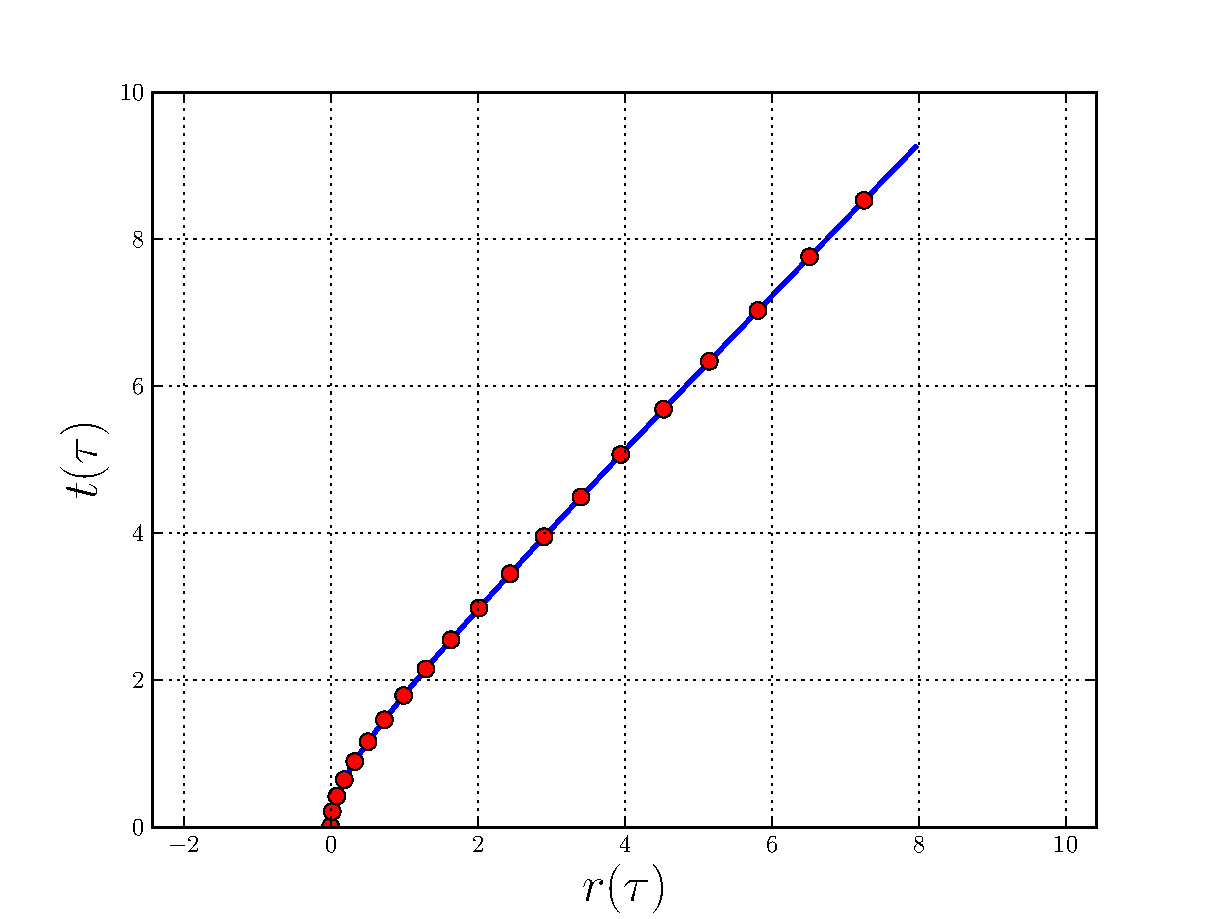
\includegraphics{minkowski.pdf}}
\caption{Expansion Radius of Model Universe, $\f{r}{\tau}$, where $\tau$ is the time coordinate.}
\end{center}
\end{figure} 
\begin{align*}
\deriv{r}{\tau} &= \tau \\
\deriv{t}{\tau} &= \sqrt{1+\tau^{2}} \\
\f{t}{\tau} &= \half\paren{\tau\sqrt{1+\tau^{2}}+\sinh^{-1}\tau}
\end{align*}
Spatial coordinates for the model universes are given by $\rho$ a spatial radius and the angular coordinates $\theta$ and $\phi$ if required. A
visualization of the 1-D spatial dimensional manifold is shown in figure~\ref{oneDU}.
\begin{sidewaysfigure}
\centering
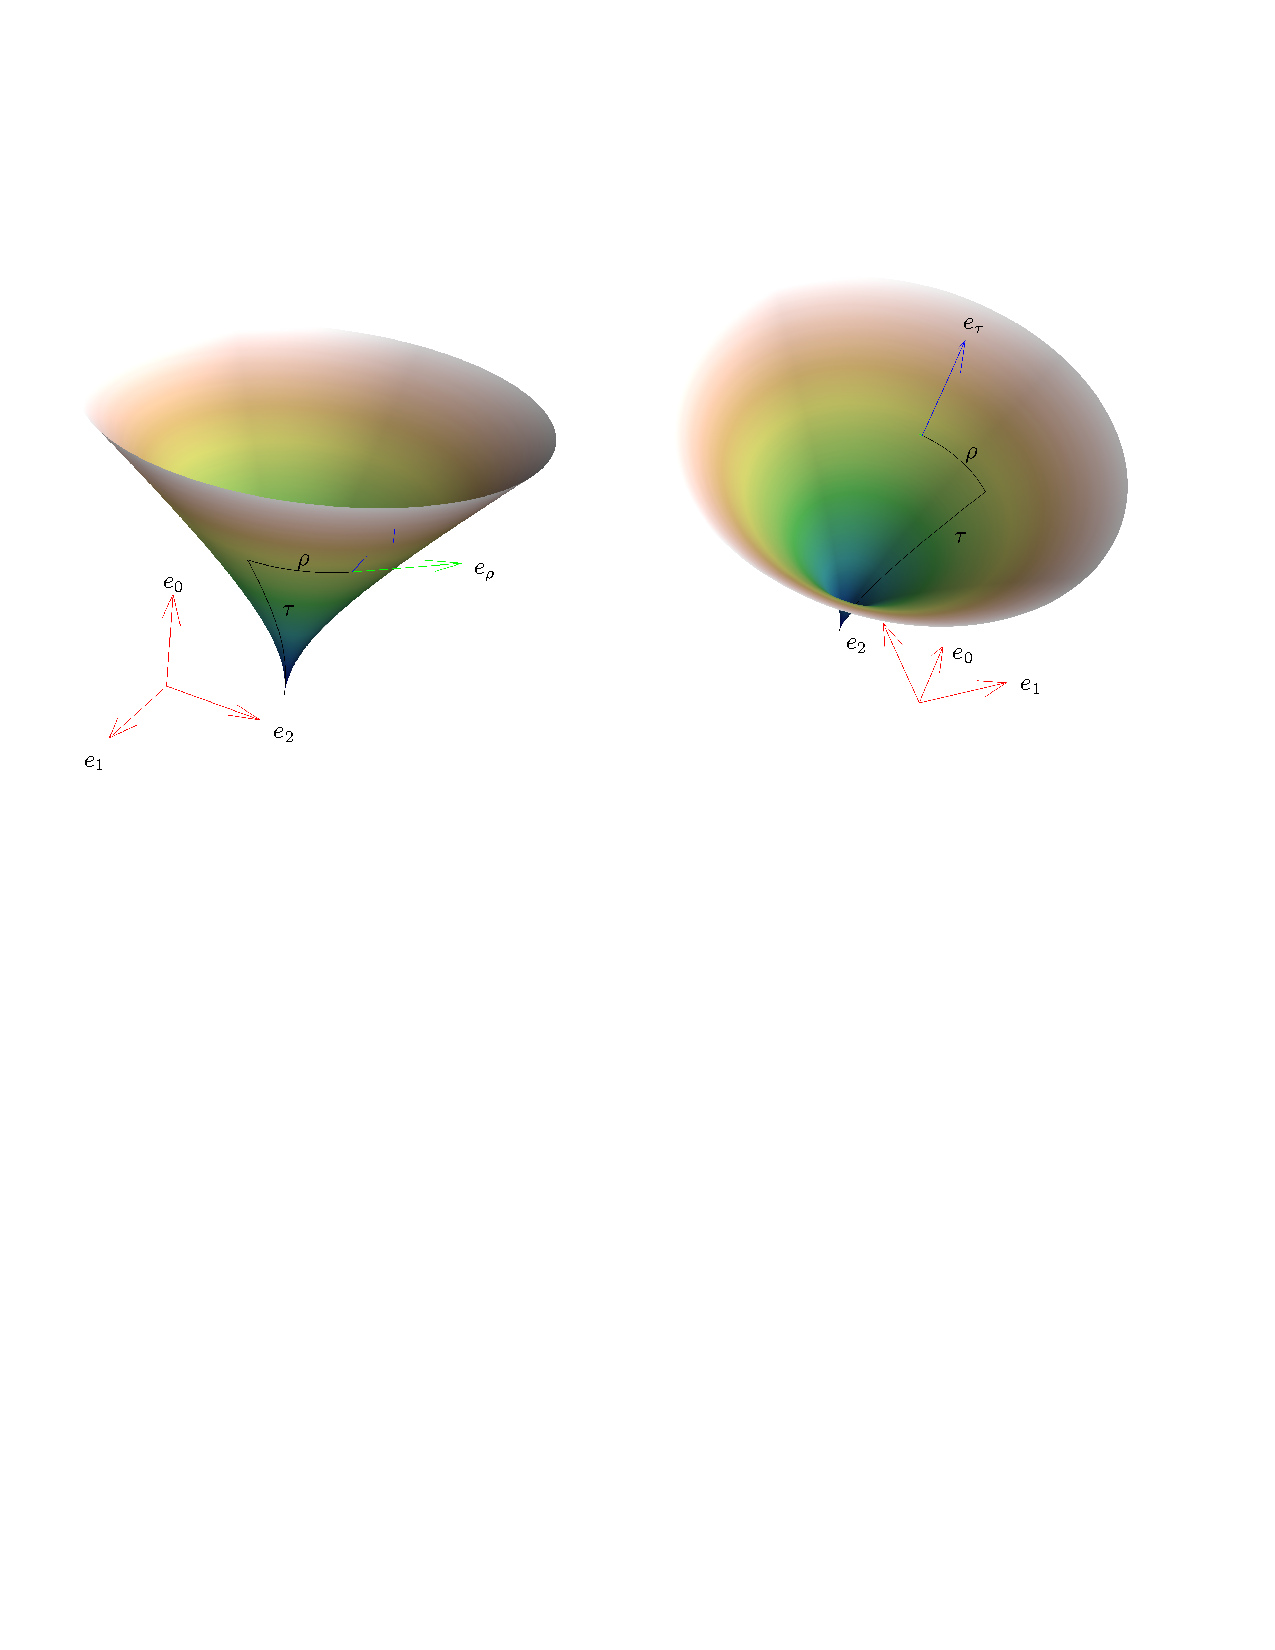
\includegraphics[clip=true,trim=0in 5in 0in 1in]{universe1d_tmp}
\caption[oneDU]{1D Universe}\label{oneDU}
\end{sidewaysfigure}
$e_{\tau}$ and $e_{\rho}$ are
\be
\begin{array}{ccc}
e_{\tau} = \pdiff{X^{(1)}}{\tau} & \mbox{ and } & e_{\rho} = \pdiff{X^{(1)}}{\rho}
\end{array}
\ee
and metric tensors for the three cases are
\be
g^{(i)}_{\mu\nu} = \pdiff{X^{(i)}}{\mu}\cdot\pdiff{X^{(i)}}{\nu}
\ee
where $\mu,\nu = \left \{ \tau,\rho,\theta,\phi \right \}$.  If we define $\f{h}{\tau,\rho}$ as
\be
 \f{h}{\tau,\rho} = \deriv{r}{\tau}\bfrac{\rho}{\f{r}{\tau}} 
\ee
Then the differential arclength given by the metric tensor, $g_{\mu\nu}$, is
\be
	\paren{ds}^{2} = g_{\mu\nu}dx^{\mu}dx^{\nu}
\ee
and the metric tensors for the three cases are (using sympy to do the algebra)
\be
g^{(1)}_{\mu\nu} = \lp
\begin{array}{cc}
1-h^{2} & h \\
h & -1 
\end{array}\rp
\ee
\be
g^{(2)}_{\mu\nu} = \lp
\begin{array}{ccc}
1-h^{2} & h & 0 \\
h & -1 & 0 \\
0 & 0 & -\paren{r\sinr}^{2} 
\end{array}\rp
\ee
\be
g^{(3)}_{\mu\nu} = \lp
\begin{array}{cccc}
1-h^{2} & h & 0 & 0 \\
h & -1 & 0 & 0 \\
0 & 0 & -\paren{r\sinr}^{2} & 0 \\
0 & 0 & 0 & -\paren{r\sinr\sin\theta}^{2} 
\end{array}\rp.
\ee
If we renormalize $e_{\theta}$ and $e_{\phi}$ to be unit vectors
\be
 e'_{\theta} = \bfrac{e_{\theta}}{\abs{r\sinr}} 
\ee
\be
 e'_{\phi} = \bfrac{e_{\phi}}{\abs{r\sinr\sin\theta}}
\ee
The metric tensors $g^{(2)}_{\mu\nu}$ and $g^{(3)}_{\mu\nu}$ become
\be
g'^{(2)}_{\mu\nu} = \lp
\begin{array}{ccc}
1-h^{2} & h & 0 \\
h & -1 & 0 \\
0 & 0 & -1 
\end{array}\rp
\ee
\be
g'^{(3)}_{\mu\nu} = \lp
\begin{array}{cccc}
1-h^{2} & h & 0 & 0 \\
h & -1 & 0 & 0 \\
0 & 0 & -1 & 0 \\
0 & 0 & 0 & -1 
\end{array}\rp
\ee
and
\be
\det\paren{g^{(1)}_{\mu\nu}} = \det\paren{g'^{(2)}_{\mu\nu}} = \det\paren{g'^{(3)}_{\mu\nu}} = -1 = I^{2}
\ee
For the 1-Dimensional space the differential arc length is
\be
 \paren{ds}^{2} = \paren{1-h^{2}}\paren{d\tau}^{2}+2hd\tau d\rho+\paren{d\rho}^{2}
\ee
so that for the light cone, $ds = 0$, we have the differential equation
\be
1-h^{2}+2h\deriv{\rho}{\tau}+\paren{\deriv{\rho}{\tau}}^{2} = 0
\ee
Note that this equation also applies to the 2 and 3 dimensional case if we set $\deriv{\theta}{\tau} = \deriv{\phi}{\tau} = 0$.  
Solving for $\deriv{\rho}{\tau}$ gives
\be\label{eq409}
	\deriv{\rho}{\tau} = h \pm 1 = \bfrac{1}{r}\deriv{r}{\tau}\rho \pm 1 = \paren{\deriv{}{\tau}\f{\ln}{r}}\rho \pm 1
\ee
Using the integration factor for linear first order differential equations the solution to equation ~\ref{eq409} is $\paren{\f{\rho}{\tau_{0}}=0}$
\be\label{eq407}
 \f{\rho}{\tau} = \pm \f{r}{\tau}\int_{\tau_{0}}^{\tau}\bfrac{d\tau'}{\f{r}{\tau'}}
\ee
Note that $\f{r}{\tau}$ and $\alpha\f{r}{\tau}$ have the same solution $\f{\rho}{\tau}$. Now consider the case that $\f{r}{\tau} = \tau^{\eta}$, then
\be
 \f{\rho}{\tau} = \pm\tau^{\eta}\int_{\tau_{0}}^{\tau} \paren{\tau'}^{-\eta}d\tau' = \lb 
\begin{array}{cc}
 \eta = 1, & \pm \tau\f{\ln}{\bfrac{\tau}{\tau_{0}}} \\
 \eta \neq 1, & \bfrac{\pm 1}{1-\eta}\paren{\tau-\tau_{0}\paren{\bfrac{\tau}{\tau_{0}}}^{\eta}} 
\end{array} 
  \rb
\ee
Typical $\f{\rho}{\tau}$'s for various $-1.5 \le \eta \le 1.5$ are shown in the light cone plot. If $\eta > 0$ the speed of light
is greater than $c$ in flat space.  If $\eta < 0$ the speed of light is less than $c$ in flat space. Note that if the universe is
curved, but not expanding or contracting the speed of light is the same as $c$ in flat space.

\begin{figure}[htbp]
\begin{center}
\scalebox{0.5}{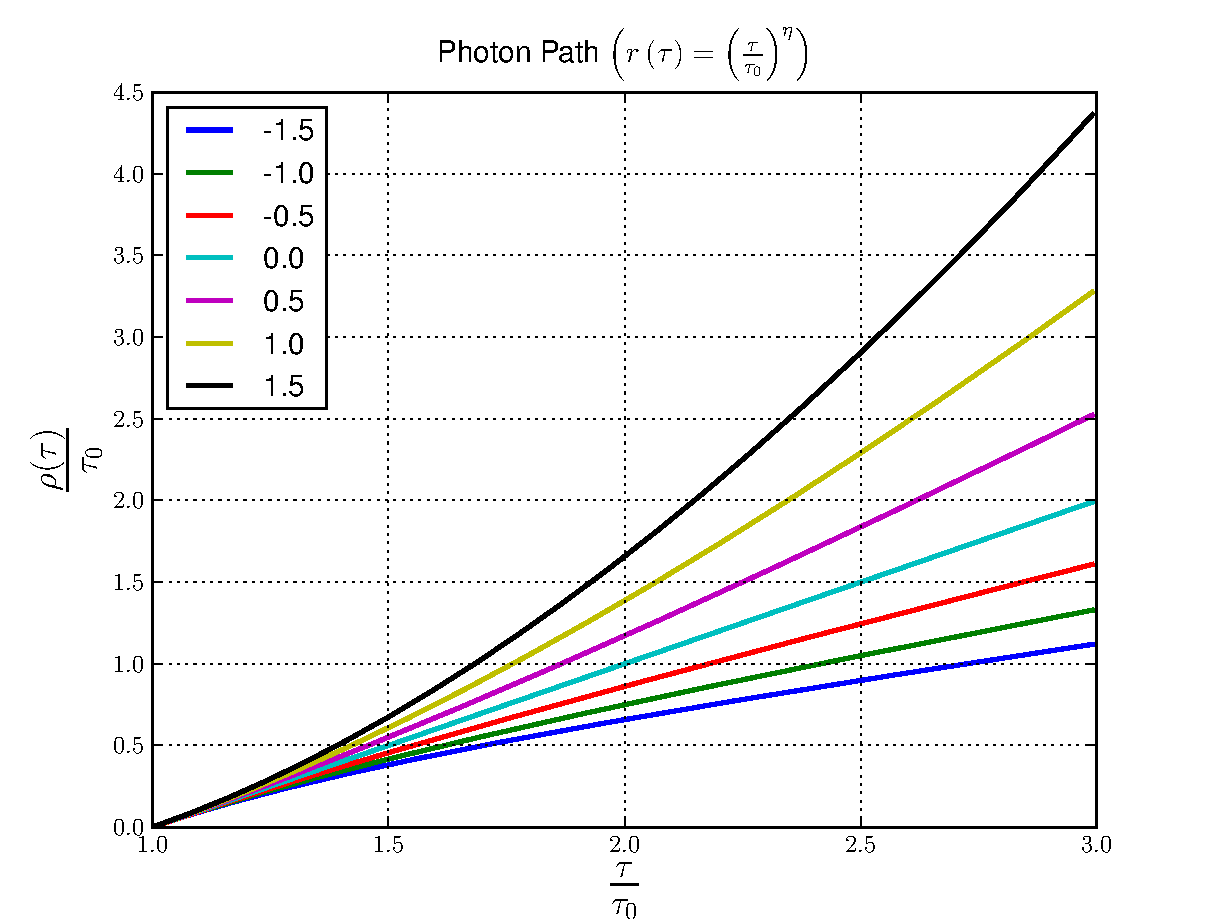
\includegraphics{lightcone.pdf}}
\caption{Lightcone in Curved Space}
\end{center}
\end{figure}
For a time periodic universe $\f{r}{\tau} = \f{\sin}{\bfrac{\tau}{T}}$ where $T$ is twice the period of the universe and $\f{\rho}{\tau_{0}}=0$, then
\be\label{eq412}
 \f{\rho}{\tau} = T\f{\sin}{\bfrac{\tau}{T}}\ln\abs{\bfrac{\f{\csc}{\bfrac{\tau_{0}}{T}}+\f{\cot}{\bfrac{\tau_{0}}{T}}}
                  {\f{\csc}{\bfrac{\tau}{T}}+\f{\cot}{\bfrac{\tau}{T}}}}
\ee
The plot of equation~\ref{eq412} is shown in figure~\ref{periodicU}
\begin{figure}[htbp]
\begin{center}
\scalebox{0.5}{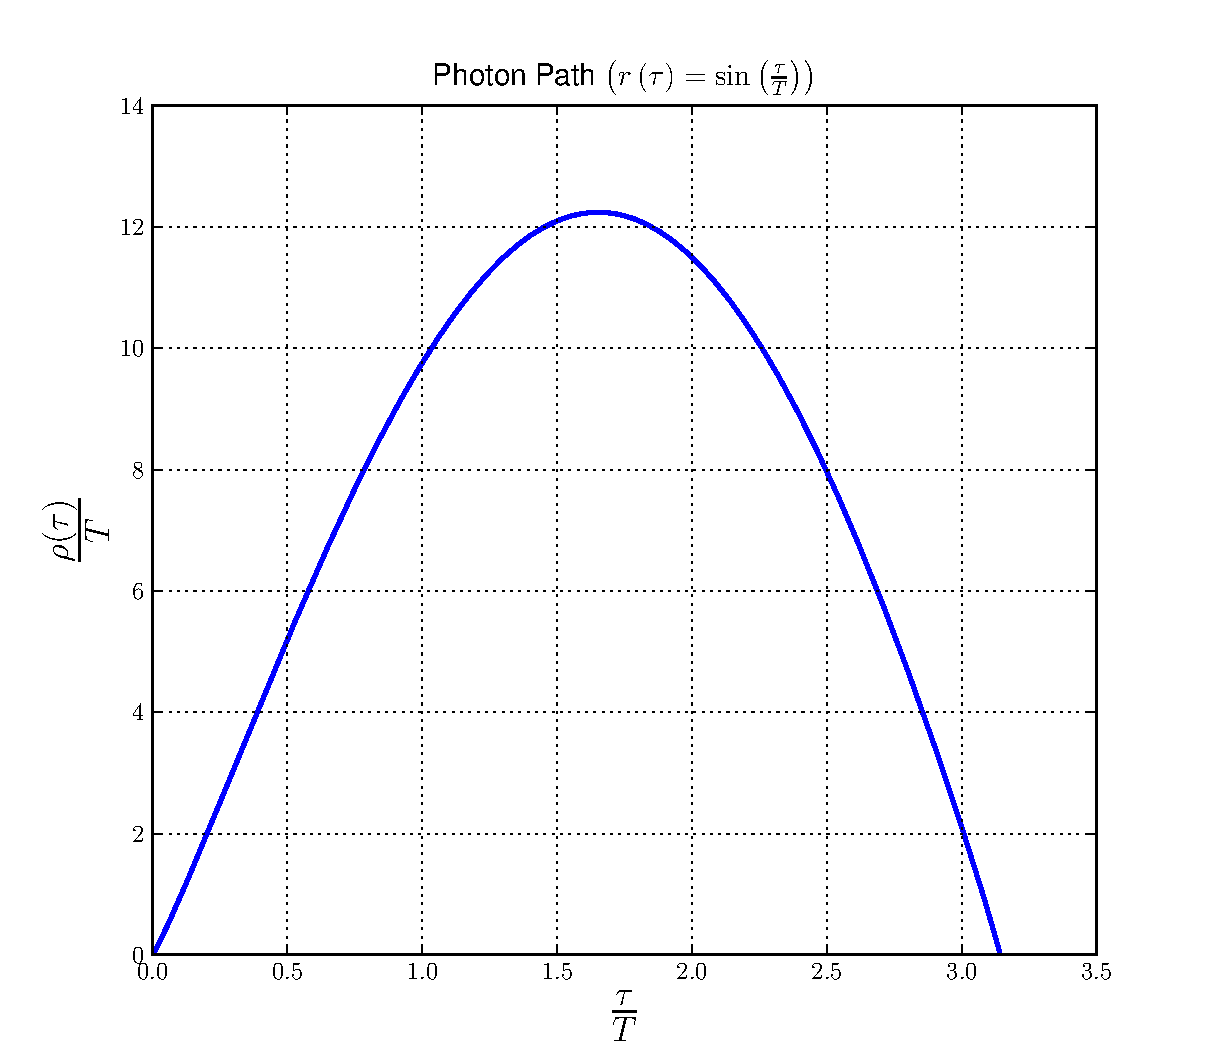
\includegraphics{periodiclightcone.pdf}}
\caption{Periodic Light Cone}\label{periodicU}
\end{center}
\end{figure}
\section{The Edge of Known Space}
Another kinematic question to answer is under what conditions light cannot access parts of the universe. The critical quantity is 
\be\label{eq410}
\f{\lambda}{\tau} = \bfrac{\f{\rho}{\tau}}{\vartheta\f{r}{\tau}}
\ee
where $\vartheta$ (the angular distance around the universe restricted to $0\le\vartheta\le\pi$) is the measure of how far from 
the observer you are. Since the universe is
spatially periodic the maximum value of $\vartheta$ is $\pi$.  If $\f{\lambda}{\tau} \ge 1$ for some finite $\tau$ you can access the 
distance defined by $\vartheta$.  Substituting equation~\ref{eq407} into equation~\ref{eq410} gives
\be
 \f{\lambda}{\tau} = \bfrac{1}{\vartheta}\int_{\tau_{0}}^{\tau}\bfrac{d\tau'}{\f{r}{\tau'}}
\ee
so that the connection condition is
\be
 \int_{\tau_{0}}^{\tau}\bfrac{d\tau'}{\f{r}{\tau'}} \ge \vartheta.
\ee
First consider a linear expansion model of the form 
\be
\f{r}{\tau} = r_{0}\paren{1+\alpha\paren{\bfrac{\tau}{\tau_{0}}-1}}
\ee
where $\f{r}{\tau_{0}} = r_{0}$.  Then
\be
\bfrac{\tau}{\tau_{0}} \ge \bfrac{1}{\alpha}e^{\alpha\vartheta\paren{\bfrac{r_{0}}{\tau_{0}}}}-1
\ee

In a linearly expanding universe the photon time of flight increases exponentially with distance. Now consider super-linear expansion of the form 
($\eta > 1$)
\be
\f{r}{\tau} = r_{0}\paren{1+\alpha\paren{\frac{\tau}{\tau_{0}}-1}^{\eta}}
\ee
Then
\be\label{eq416}
\bfrac{\tau_{0}}{r_{0}}\alpha^{-\frac{1}{\eta}}\int_{0}^{\alpha^{\frac{1}{\eta}}\paren{\frac{\tau}{\tau_{0}}-1}}\frac{d\mu}{1+\mu^{\eta}} \ge \vartheta,
\ee
but the integral in equation~\ref{eq416} does not have a closed form solution unless we let $\tau\rightarrow\infty$.  In that 
case\footnote{$\int_{0}^{\infty}\frac{dx}{1+x^{\eta}}$ is 3.241-2 in "Gradshteyn and Ryzhik"} we can write
\be\label{eq417}
\frac{1}{\eta}\alpha^{-\frac{1}{\eta}}\f{\csc}{\frac{\pi}{\eta}} \ge \paren{\frac{\vartheta}{\pi}}\paren{\frac{r_{0}}{\tau_{0}}}
\ee
A contour plot of the left side of equation~\ref{eq417} is shown below

\begin{figure}[htbp]
\begin{center}
\scalebox{0.5}{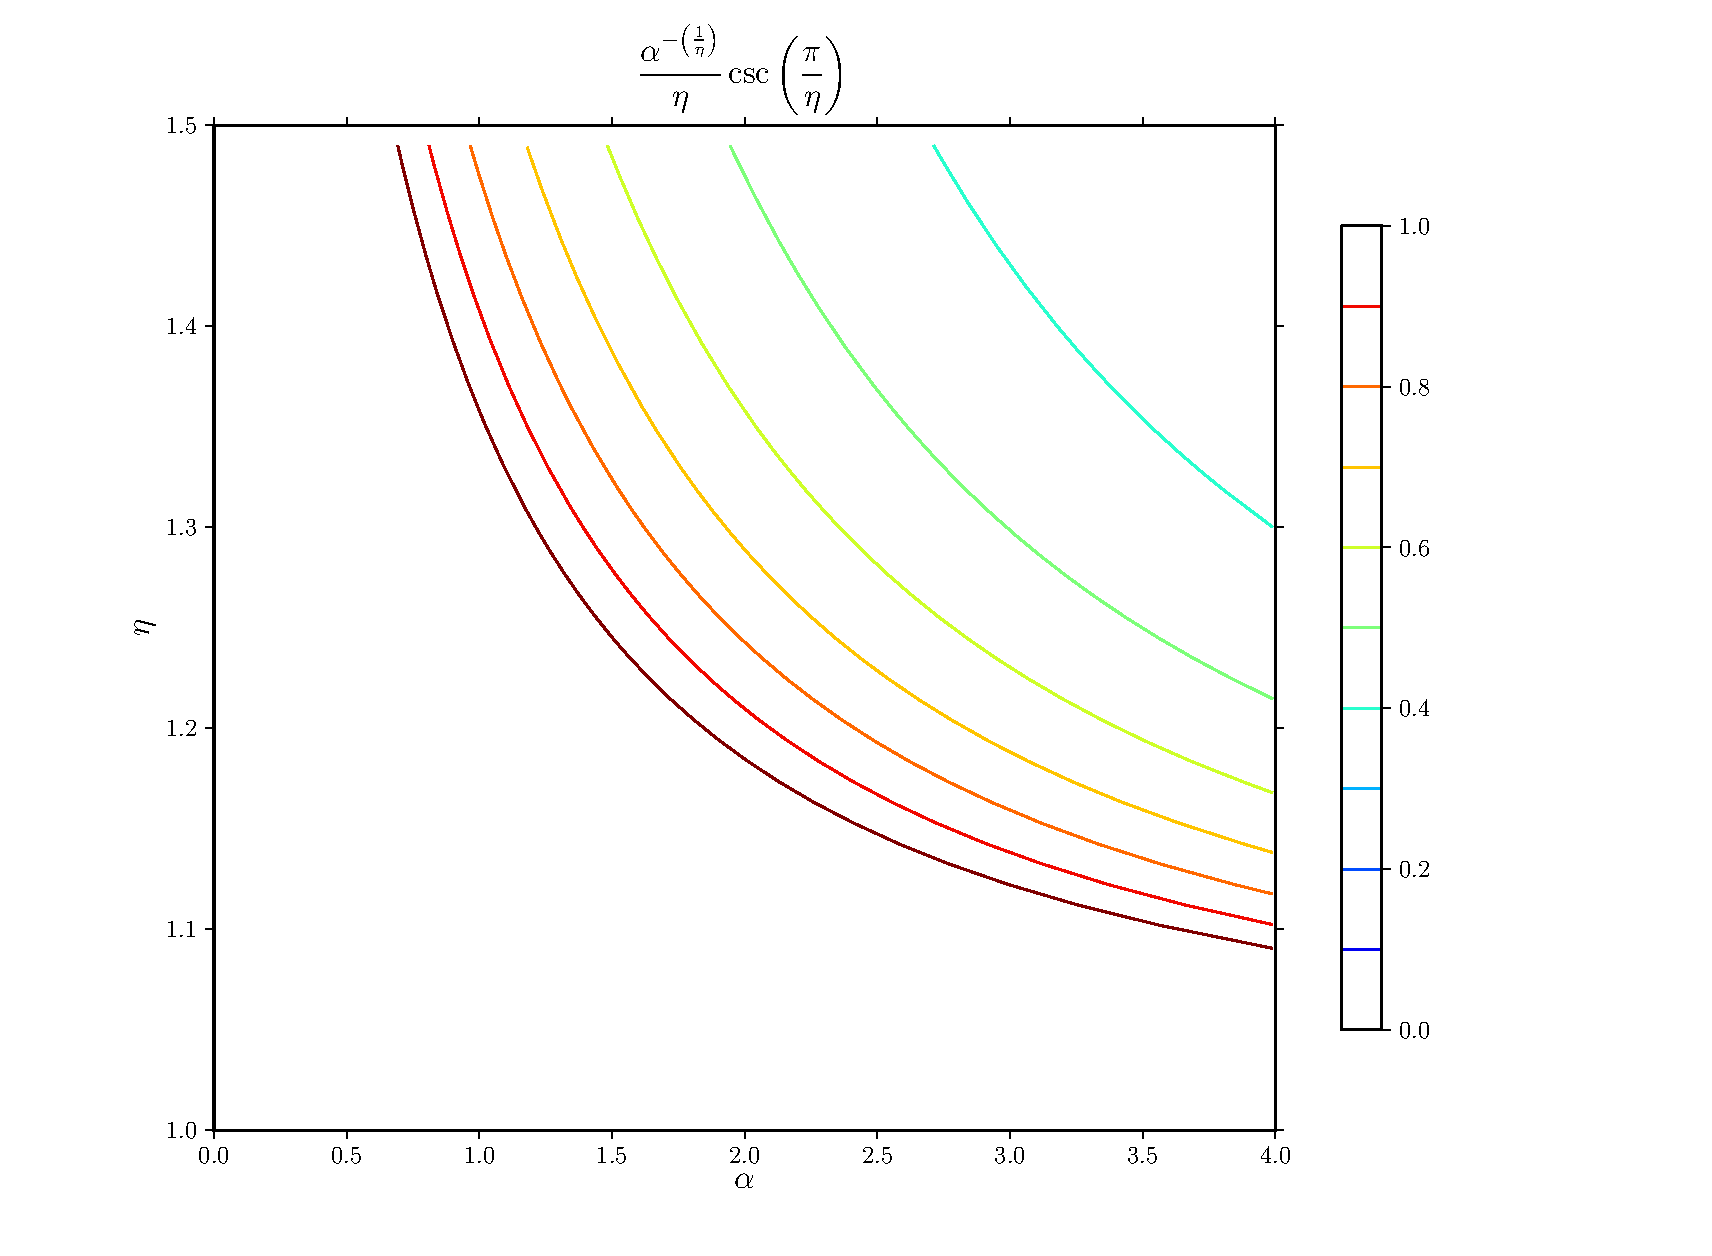
\includegraphics{exclusion.pdf}}
\caption{Photon Exclusion Zone}
\end{center}
\end{figure}
The right side of equation~\ref{eq417}, $\paren{\bfrac{\vartheta}{\pi}}\paren{\bfrac{r_{0}}{\tau_{0}}}$, is interpreted as follows -
\begin{enumerate}
 \item $\bfrac{\vartheta}{\pi}$ is the fractional distance around the closed spatially periodic universe. $\bfrac{\vartheta}{\pi}=1$ is as far as one can
 go before the distance from the observer starts to decrease.
 \item $\bfrac{r_{0}}{\tau_{0}}$ is a measure of inflation.  Immediately after an inflationary epoch $\bfrac{r_{0}}{\tau_{0}} >> 1$.
\end{enumerate}
Thus equation~\ref{eq417} determined the maximum distance $\bfrac{\vartheta}{\pi}$ that a photon can propagate in a finite amount of time.

Another question to consider is under what conditions $\bfrac{r_{0}}{\tau_{0}}$ will increase as $\tau_{0}$ increases or when will the
following be true
\be\label{eq418}
 \bfrac{\f{r}{\tau}}{\tau} \ge \bfrac{\f{r}{\tau_{0}}}{\tau_{0}} .
\ee
Equation~\ref{eq418} is equivalent to 
\be
 \alpha\paren{\bfrac{\tau}{\tau_{0}}-1}^{\eta-1} \ge 1
\ee
so that if $\eta >1$ then $\bfrac{\f{r}{\tau_{0}}}{\tau_{0}}$ will eventually grow as $\tau_{0}$ increases.
